\documentclass[11pt]{article}
\usepackage[margin=1in]{geometry}
\usepackage{amsmath,amssymb}
\usepackage{graphicx}
\usepackage{booktabs}
\usepackage{siunitx}
\usepackage{xcolor}
\usepackage[colorlinks=true,linkcolor=blue,urlcolor=blue]{hyperref}
\usepackage{caption}
\captionsetup{font=small}

\title{\vspace{-2em}On the non-smoothness of stress components in the dynamic
torsion verification problem}
\author{Alejandro Mota \\ \small Sandia National Laboratories}
\date{\today}

\newcommand{\sib}[1]{\,\mathrm{#1}}

\begin{document}
\maketitle
\vspace{-1.5em}

\section*{Summary}
For the dynamic torsion benchmark, the individual Cauchy stress
\emph{components} ($\sigma_{xx},\sigma_{yy},\sigma_{zz}$, and to a lesser extent
the off-diagonal terms) appear ``choppy'' in space, while the von Mises stress
is smooth. This is the \emph{physically correct} behavior, not a numerical
artifact, a projection error, or a deficiency of Norma. Two facts explain it:

\begin{enumerate}\itemsep2pt
  \item \textbf{It is a strongly dynamic, wave-dominated problem.} The bar is
  set in motion by a large initial torsional velocity (corner speed
  $\approx \SI{141}{m/s}$). Elastic waves propagate and reflect off the free
  ends throughout the simulation. The small normal stress components are
  dominated by these traveling waves and therefore oscillate in space.
  \item \textbf{The response is shear-dominated.} The twisting generates shear
  stresses $\approx \SI{87}{MPa}$, an order of magnitude larger than the normal
  components ($\sim\SI{6}{MPa}$). Von Mises is governed by the (smooth, large)
  shear and is essentially blind to the (small, oscillatory) normal components.
\end{enumerate}

\noindent We confirm this with a four-code verification: \textbf{Norma},
\textbf{Carina}, \textbf{LCM/Albany}, and \textbf{Sierra/Adagio} all reproduce
the same behavior on the same mesh, with peak von Mises agreeing to within
$3\%$ (Norma and Carina agree to machine precision). The choppiness is present
in \emph{every} code; it is physics, not a bug.

\section{The problem is highly dynamic}
A $0.05\times0.05\times1.0\sib{m}$ Neo-Hookean bar ($E=\SI{1}{GPa}$, $\nu=0.25$,
$\rho=\SI{1000}{kg/m^3}$), free at both ends, is given the initial torsional
velocity field $v_x=-a\,y\,z$, $v_y=a\,x\,z$, $v_z=0$ with
$a=8000\sib{(m\,s)^{-1}}$ (so that $a$ multiplied by two lengths yields a
velocity). It is integrated implicitly (Newmark, $\beta=0.25$, $\gamma=0.5$,
$\Delta t=\SI{1}{\micro s}$) to $t=\SI{2}{ms}$.

The initial velocity is large: at a top corner ($z=0.5$),
$|\mathbf v| = \sqrt{2}\,a\,(0.025)(0.5) \approx \SI{141}{m/s}$. The bar twists
through roughly half a turn end-to-end at maximum deformation. The relevant
wave speeds are
\begin{equation}
  c_s=\sqrt{G/\rho}=\SI{632}{m/s},\qquad
  c_p=\sqrt{(K+\tfrac{4}{3}G)/\rho}=\SI{1095}{m/s},
\end{equation}
with $G=\SI{4.0e8}{Pa}$, $K=\SI{6.67e8}{Pa}$. Over the bar length $L=\SI{1}{m}$
these give transit times $L/c_s=\SI{1.58}{ms}$ and $L/c_p=\SI{0.91}{ms}$, so in
the $\SI{2}{ms}$ window the shear and dilatational fronts cross the bar
$\sim\!1.3$ and $\sim\!2.2$ times, respectively, reflecting repeatedly off the
free ends. \emph{The bar is full of propagating, reflecting elastic waves at all
times.}

\section{Why the stress components are non-smooth}
In pure (small-strain) torsion the only nonzero stresses are shears; the normal
components vanish. Here the normal components $\sigma_{xx},\sigma_{yy},
\sigma_{zz}$ are nonzero only through (i) finite-deformation coupling
(second order in the twist) and (ii) the axial/dilatational waves launched by
the impulsive start and the free-end reflections. They are therefore both
\emph{small} ($\sim\!\SI{1}{}$–$\SI{6}{MPa}$) and \emph{dominated by traveling
waves}. A wave field sampled at a single instant is spatially oscillatory by
nature --- the ``choppiness'' is the snapshot of wavefronts moving through the
bar. Because the normal components have no large, smooth mean value to sit on,
the wave ripple \emph{is} the entire signal, so it is fully visible.

\section{Why von Mises is smooth}
The von Mises stress is
\begin{equation}
  \sigma_{\mathrm{vM}}
  =\sqrt{\tfrac12\!\left[(\sigma_{xx}-\sigma_{yy})^2+(\sigma_{yy}-\sigma_{zz})^2
  +(\sigma_{zz}-\sigma_{xx})^2\right]+3\!\left(\sigma_{xy}^2+\sigma_{yz}^2
  +\sigma_{xz}^2\right)}.
\end{equation}
At peak deformation $\sigma_{\mathrm{vM}}\approx\SI{150}{MPa}$, which for this
shear-dominated state corresponds to a shear magnitude
$\tau\approx\sigma_{\mathrm{vM}}/\sqrt3\approx\SI{87}{MPa}$. The shear term
$3\tau^2$ thus exceeds the normal-difference term by roughly three orders of
magnitude ($3\cdot87^2$ vs.\ a few $\times\,6^2$, in $\si{MPa^2}$). Since
$\sigma_{\mathrm{vM}}$ scales with the \emph{square} of the components, the
small oscillatory normal stresses perturb it by well under $1\%$. Von Mises
therefore tracks the large, smooth, twist-driven shear and looks smooth ---
exactly as observed. This is a property of the quantity, not evidence that the
components are ``more accurate'' than von Mises or vice versa.

\section{Is it the coarse mesh?}
The mesh ($2\times2\times40$ hexes) is coarse, and that does set the
\emph{granularity} of what is plotted: the raw quadrature-point values are
piecewise discontinuous between elements (hence the blockiest pictures), and a
coarse mesh resolves only the longer-wavelength waves, aliasing the shorter
ones. The $L^2$ projection to nodes removes the inter-element jumps but cannot
manufacture sub-element information, so the projected normal components still
show the underlying oscillation. Crucially, this is \emph{resolution}, not
\emph{error}: refining the mesh would resolve the waves more finely (more, and
crisper, wavefronts) and converge to the true wave-filled solution --- it would
not flatten the components to zero, because the oscillation is real. The
clinching evidence is in the next section: four independent codes on this
\emph{same} coarse mesh produce the same fields.

\section{Four-code verification}
The identical problem was run in four independent codes on the same mesh, with
stresses projected to the nodes by $L^2$ projection and evaluated at the instant
of maximum strain energy ($t^\star=\SI{7.9e-4}{s}$).

\begin{table}[h]
\centering
\begin{tabular}{llcl}
\toprule
Code & Framework & Peak $\sigma_{\mathrm{vM}}$ [MPa] & Agreement vs.\ Norma \\
\midrule
Norma  & Julia FE (reference)         & 150.0 & --- \\
Carina & Julia FE (GPU)               & 150.0 & machine precision ($\sim\!10^{-4}\sib{Pa}$) \\
LCM    & C++/Trilinos (Albany)        & 150.1 & $0.09\%$ \\
Adagio & Sierra/SolidMechanics        & 155.1 & $\sim\!3\%$ (lumped mass, see below) \\
\bottomrule
\end{tabular}
\caption{Peak nodal von Mises at $t^\star$ and node-wise agreement with Norma
(matched by reference coordinates). Norma and Carina (sibling codes, consistent
mass) agree to machine precision and LCM to $0.09\%$. Adagio's $\sim\!3\%$
difference comes from its \emph{lumped} mass matrix for implicit integration:
the lumped mass changes the rotational inertia and hence the dynamic trajectory,
so at the fixed time $t^\star$ Adagio is in a slightly different configuration.
Its stress projection is consistent --- the difference is in the
time-integration mass, not the stress.}
\end{table}

Figure~\ref{fig:lines} overlays the projected nodal fields along the bar for all
four codes. Two things are evident. First, von Mises is a smooth tent peaking at
mid-span, while the normal components are oscillatory. Second, the curves for
\textbf{Norma, Carina, and LCM lie essentially on top of one another}: the
oscillation is reproduced, to plotting accuracy, by three completely independent
implementations, so it is the physical solution and not code-specific noise.

\textbf{Adagio} shows the same qualitative pattern but is visibly offset from
the other three. This is expected, and it is \emph{not} a discrepancy in the
stress computation: Adagio uses a \emph{lumped} mass matrix for the implicit
integration, whereas the other three use the \emph{consistent} mass. The lumped
mass changes the rotational inertia of the discretization and therefore the
dynamic trajectory of the twisting bar. By the fixed sampling time $t^\star$ the
Adagio bar is consequently in a slightly different twist configuration than the
consistent-mass codes, so its instantaneous stresses are sampled at a
correspondingly different state --- which is exactly why its curves are shifted
rather than coincident. The three consistent-mass codes share the same
trajectory and so coincide. (Adagio's stress projection itself is consistent;
the difference is purely in the time-integration mass.)

Figure~\ref{fig:vm} shows the smooth von Mises field on the deformed (twisted)
bar, and Figures~\ref{fig:sxx}--\ref{fig:szz} the normal components, which
display the propagating-wave pattern. The same coincidence holds: the field is
visually identical for the three consistent-mass codes, with Adagio sampled at
its slightly different configuration.

\begin{figure}[h]
\centering
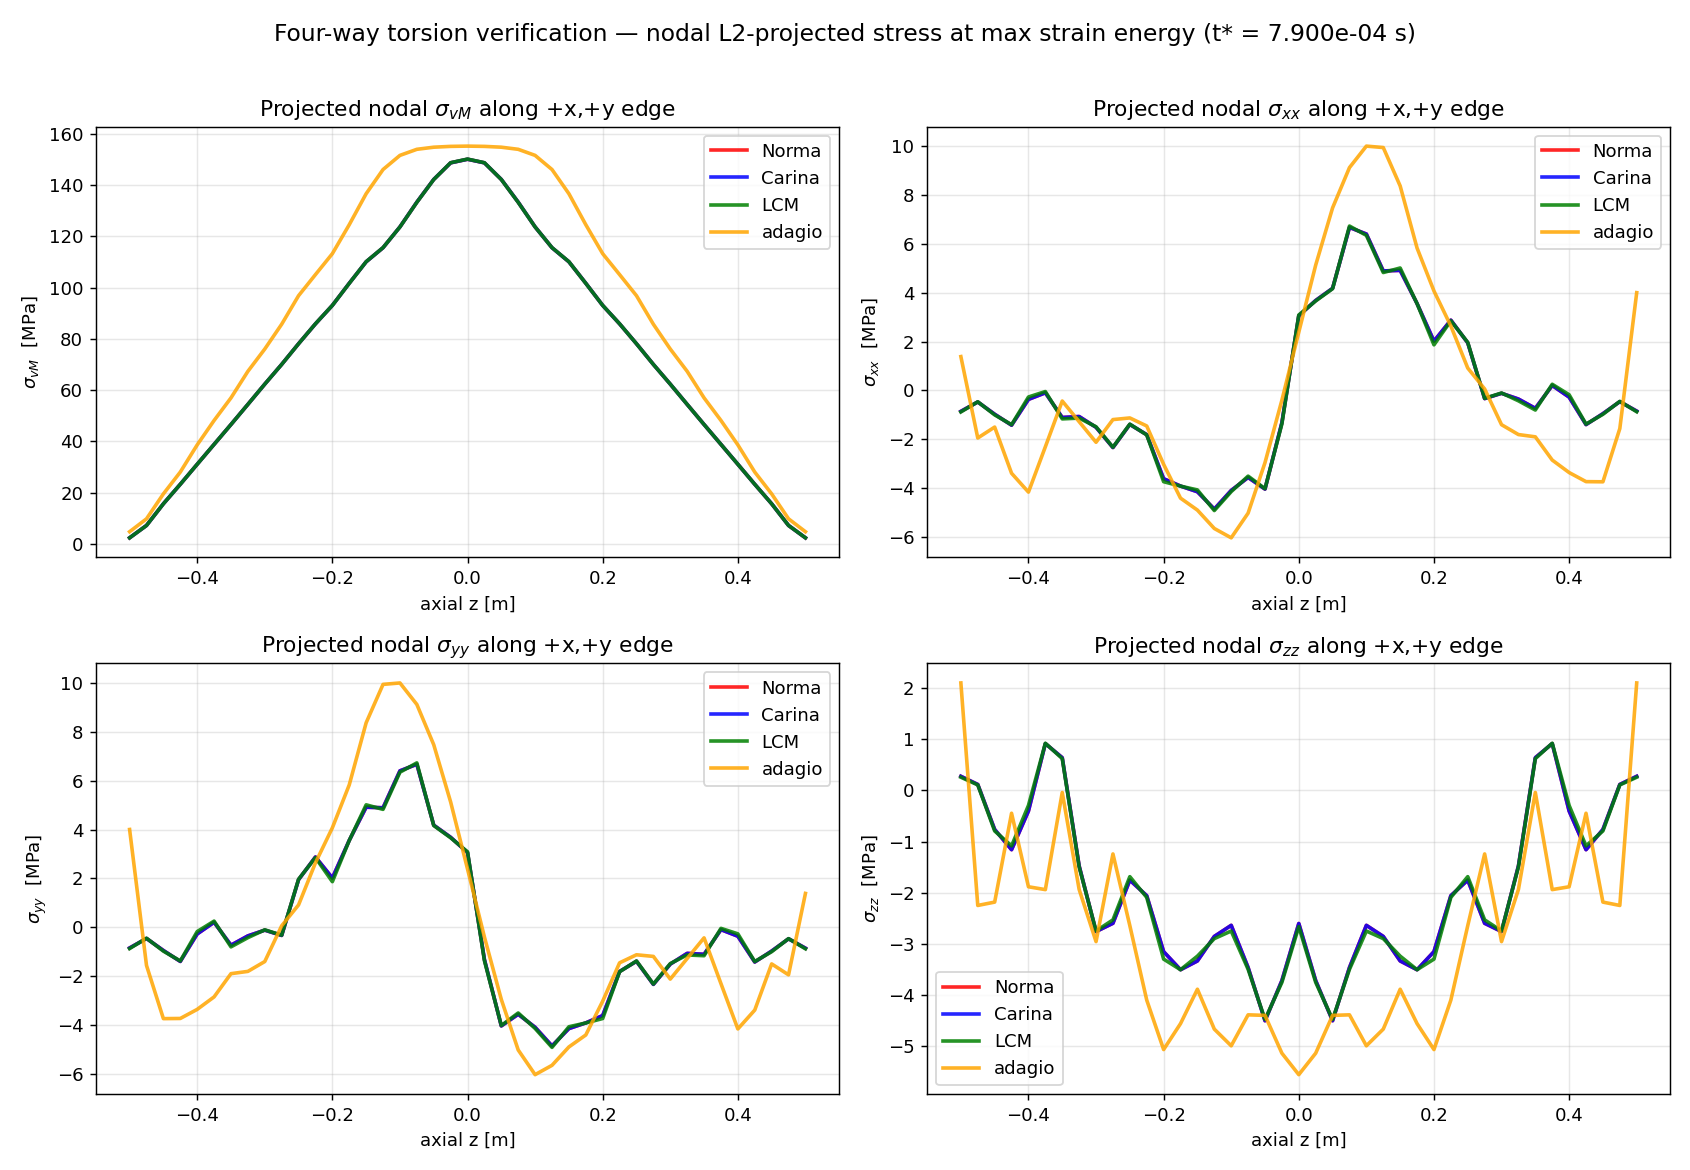
\includegraphics[width=\textwidth]{figures/axial_overlay.png}
\caption{Projected nodal stress vs.\ axial position along the bar's edge, four
codes overlaid (Norma red, Carina blue, LCM green, Adagio orange). Von Mises
(top left) is smooth; the normal components are wave-dominated and oscillatory,
yet the four codes agree.}
\label{fig:lines}
\end{figure}

\begin{figure}[hbt]
\centering
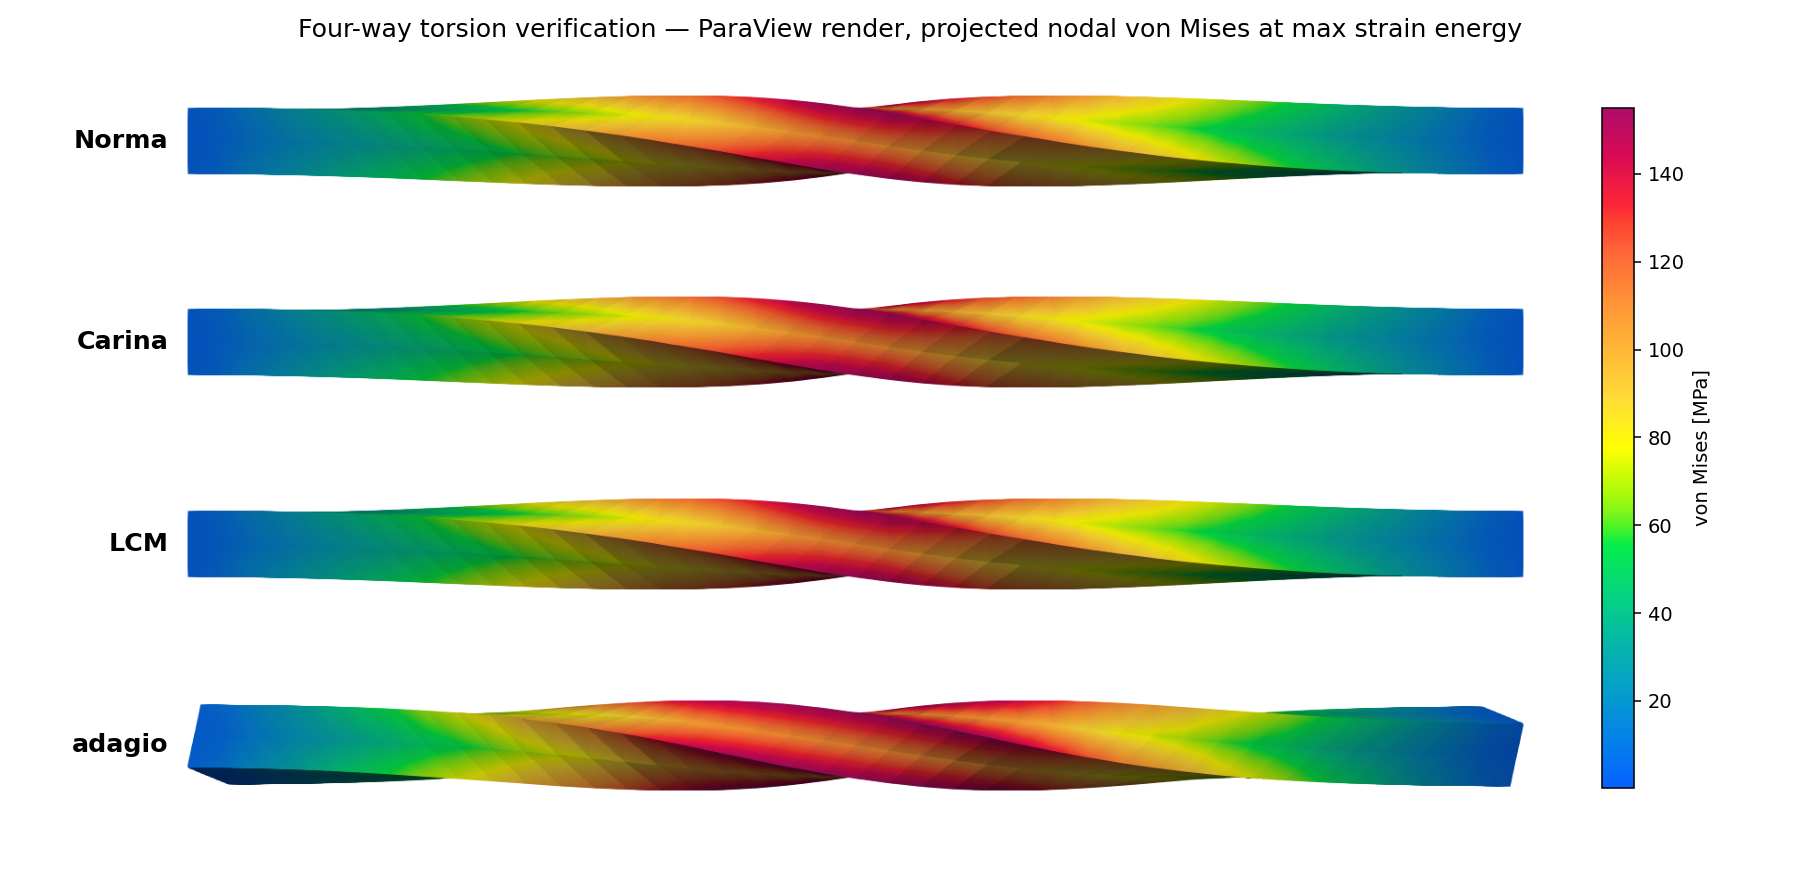
\includegraphics[width=\textwidth]{figures/pv_vm.png}
\caption{ParaView render of the twisted bar at $t^\star$ (true scale), projected
nodal von Mises, four codes stacked. The field is smooth in every code; Norma,
Carina, and LCM are visually identical, while Adagio (lumped mass) is sampled at
a slightly different configuration.}
\label{fig:vm}
\end{figure}

\begin{figure}[hbt]
\centering
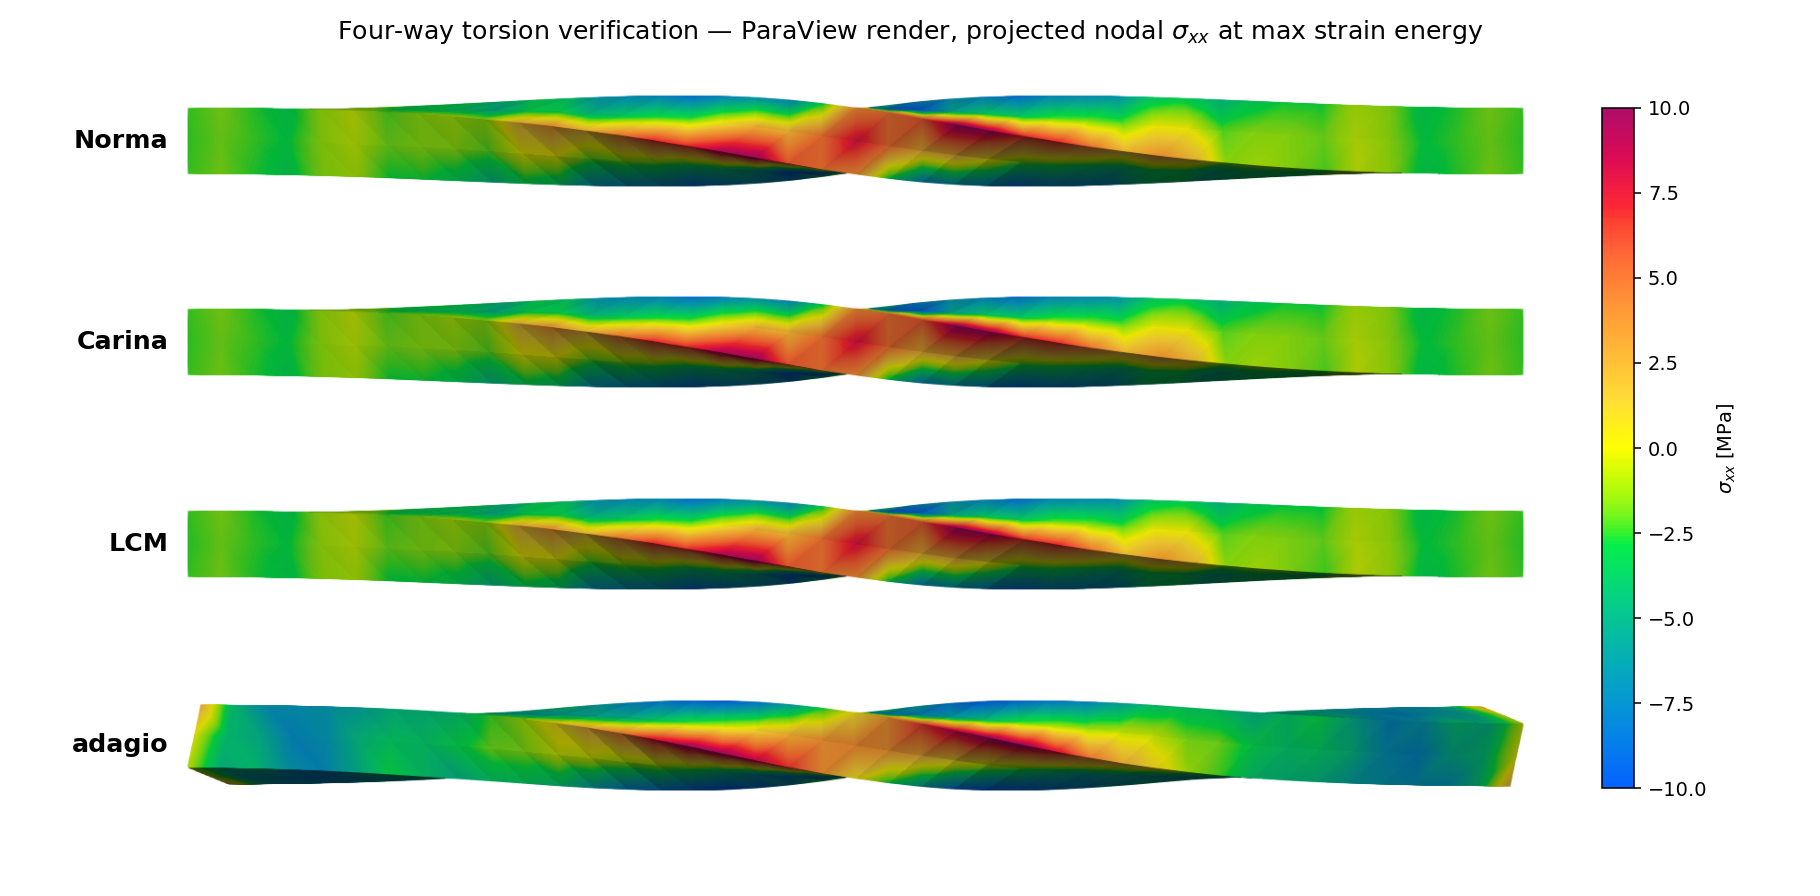
\includegraphics[width=\textwidth]{figures/pv_sxx.png}
\caption{Projected nodal $\sigma_{xx}$ on the twisted bar at $t^\star$. The
propagating-wave pattern is evident. Norma, Carina, and LCM agree; Adagio
(lumped mass) is sampled at a slightly different configuration.}
\label{fig:sxx}
\end{figure}

\begin{figure}[hbt]
\centering
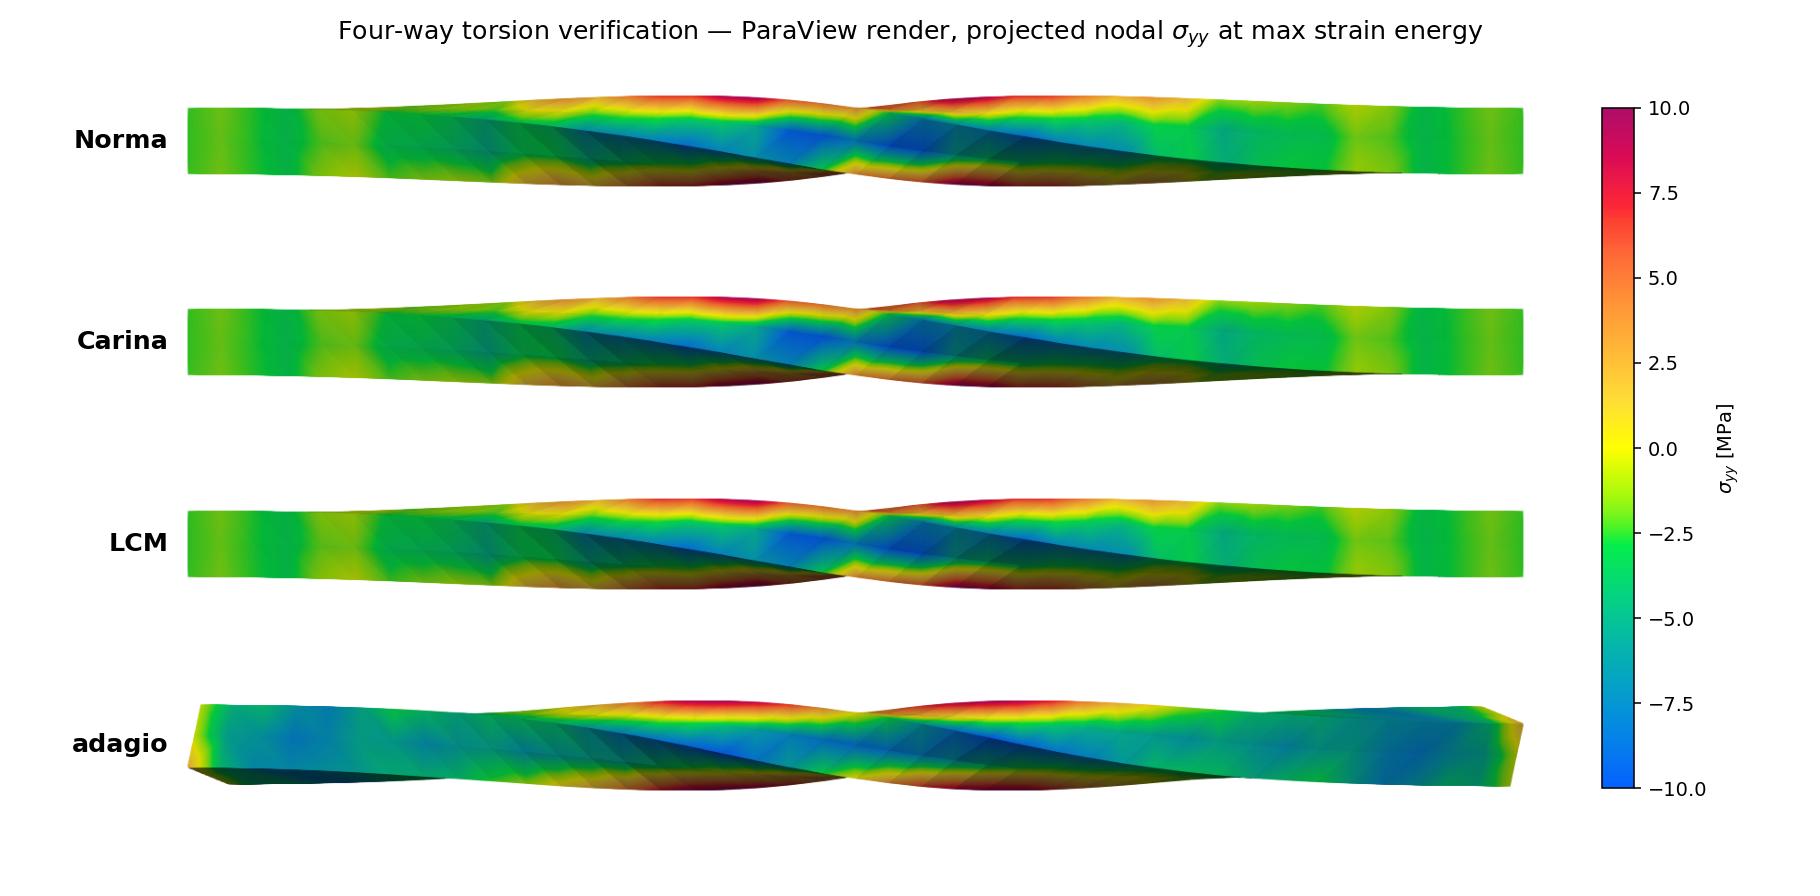
\includegraphics[width=\textwidth]{figures/pv_syy.png}
\caption{Projected nodal $\sigma_{yy}$ on the twisted bar at $t^\star$, four
codes stacked. As for $\sigma_{xx}$, the wave pattern is physical and shared by
the three consistent-mass codes.}
\label{fig:syy}
\end{figure}

\begin{figure}[hbt]
\centering
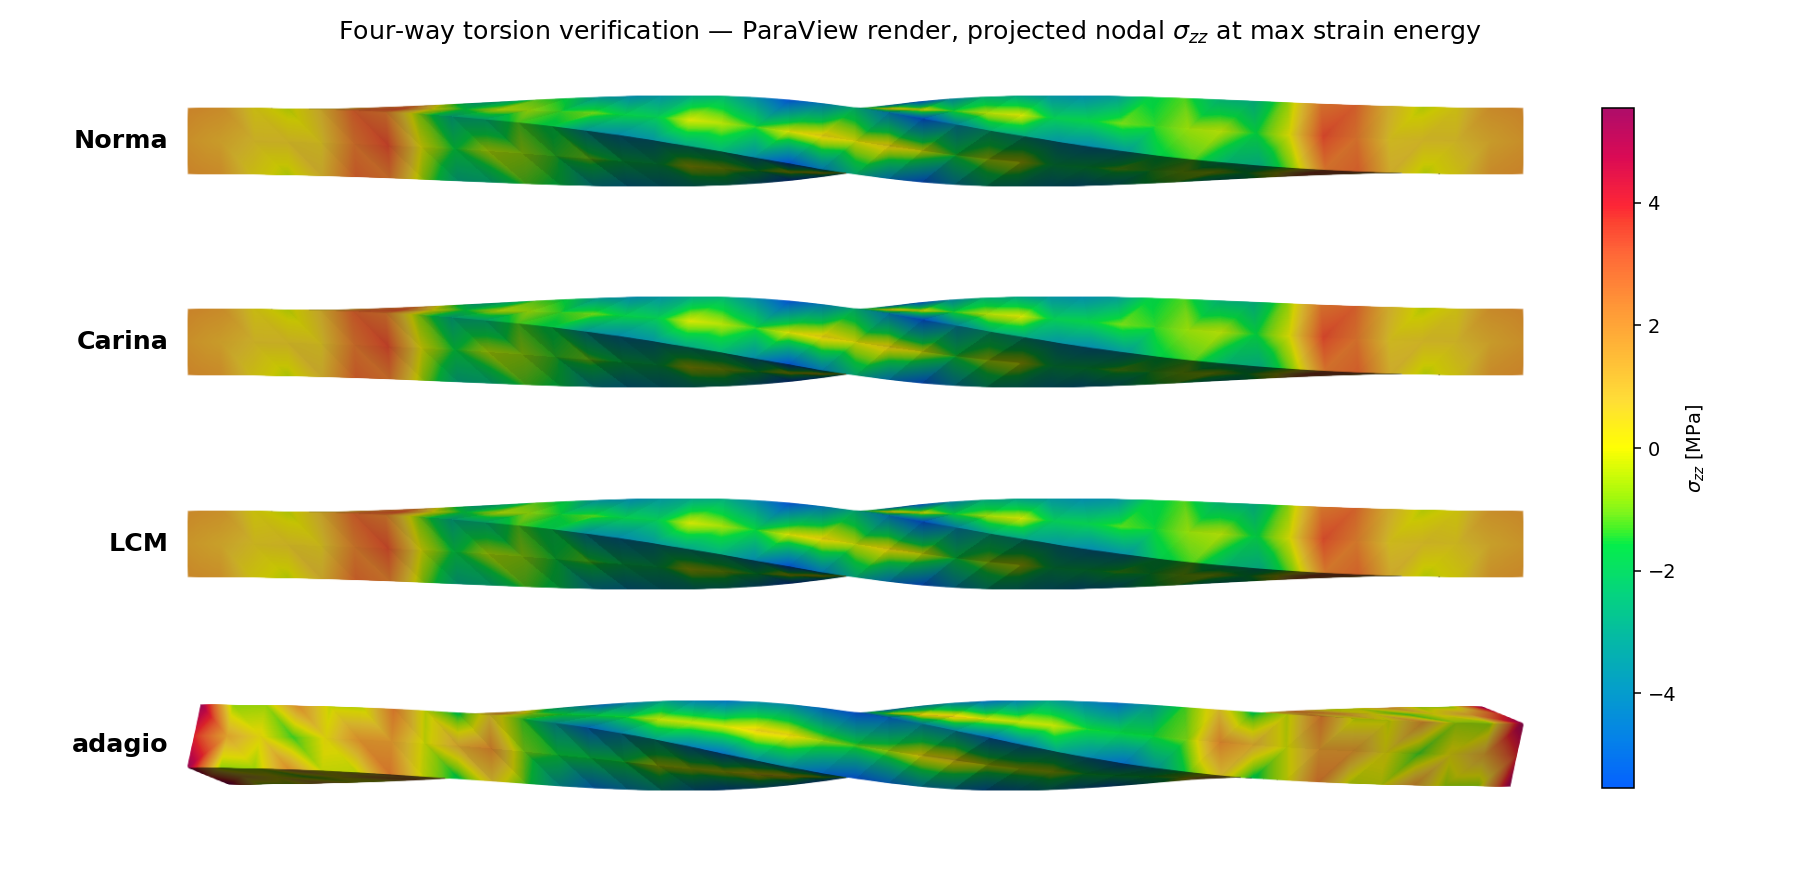
\includegraphics[width=\textwidth]{figures/pv_szz.png}
\caption{Projected nodal $\sigma_{zz}$ on the twisted bar at $t^\star$, four
codes stacked. The axial normal stress likewise reflects the dilatational waves
propagating along the bar.}
\label{fig:szz}
\end{figure}

\section{Conclusion}
The non-smoothness of the stress components is the correct physical response of
a coarse-mesh, strongly dynamic, wave-filled torsion problem; von Mises looks
smooth because the response is shear-dominated and von Mises is governed by that
large, smooth shear. Four independent codes reproduce both features on the same
mesh and agree on peak von Mises to within $3\%$ (two of them to machine
precision). None of this indicates any inaccuracy in Norma.

\end{document}
